\begin{fakeXML}[label=kml,caption=A simple KML example representing a Point]
<?xml version="1.0" encoding="UTF-8"?>
<kml xmlns="http://www.opengis.net/kml/2.2">
<document>
<placemark>
  <name>New York City</name>
  <description>New York City</description>
  <point>
    <coordinates>-74.006393,40.714172,0</coordinates>
  </point>
</placemark>
</document>
</kml>
\end{fakeXML} 

\begin{fakeJSON}[label=kml,caption=JSON Data]
{"prakash":"Thapa"}
\end{fakeJSON} 


\begin{figure}
	\centering
	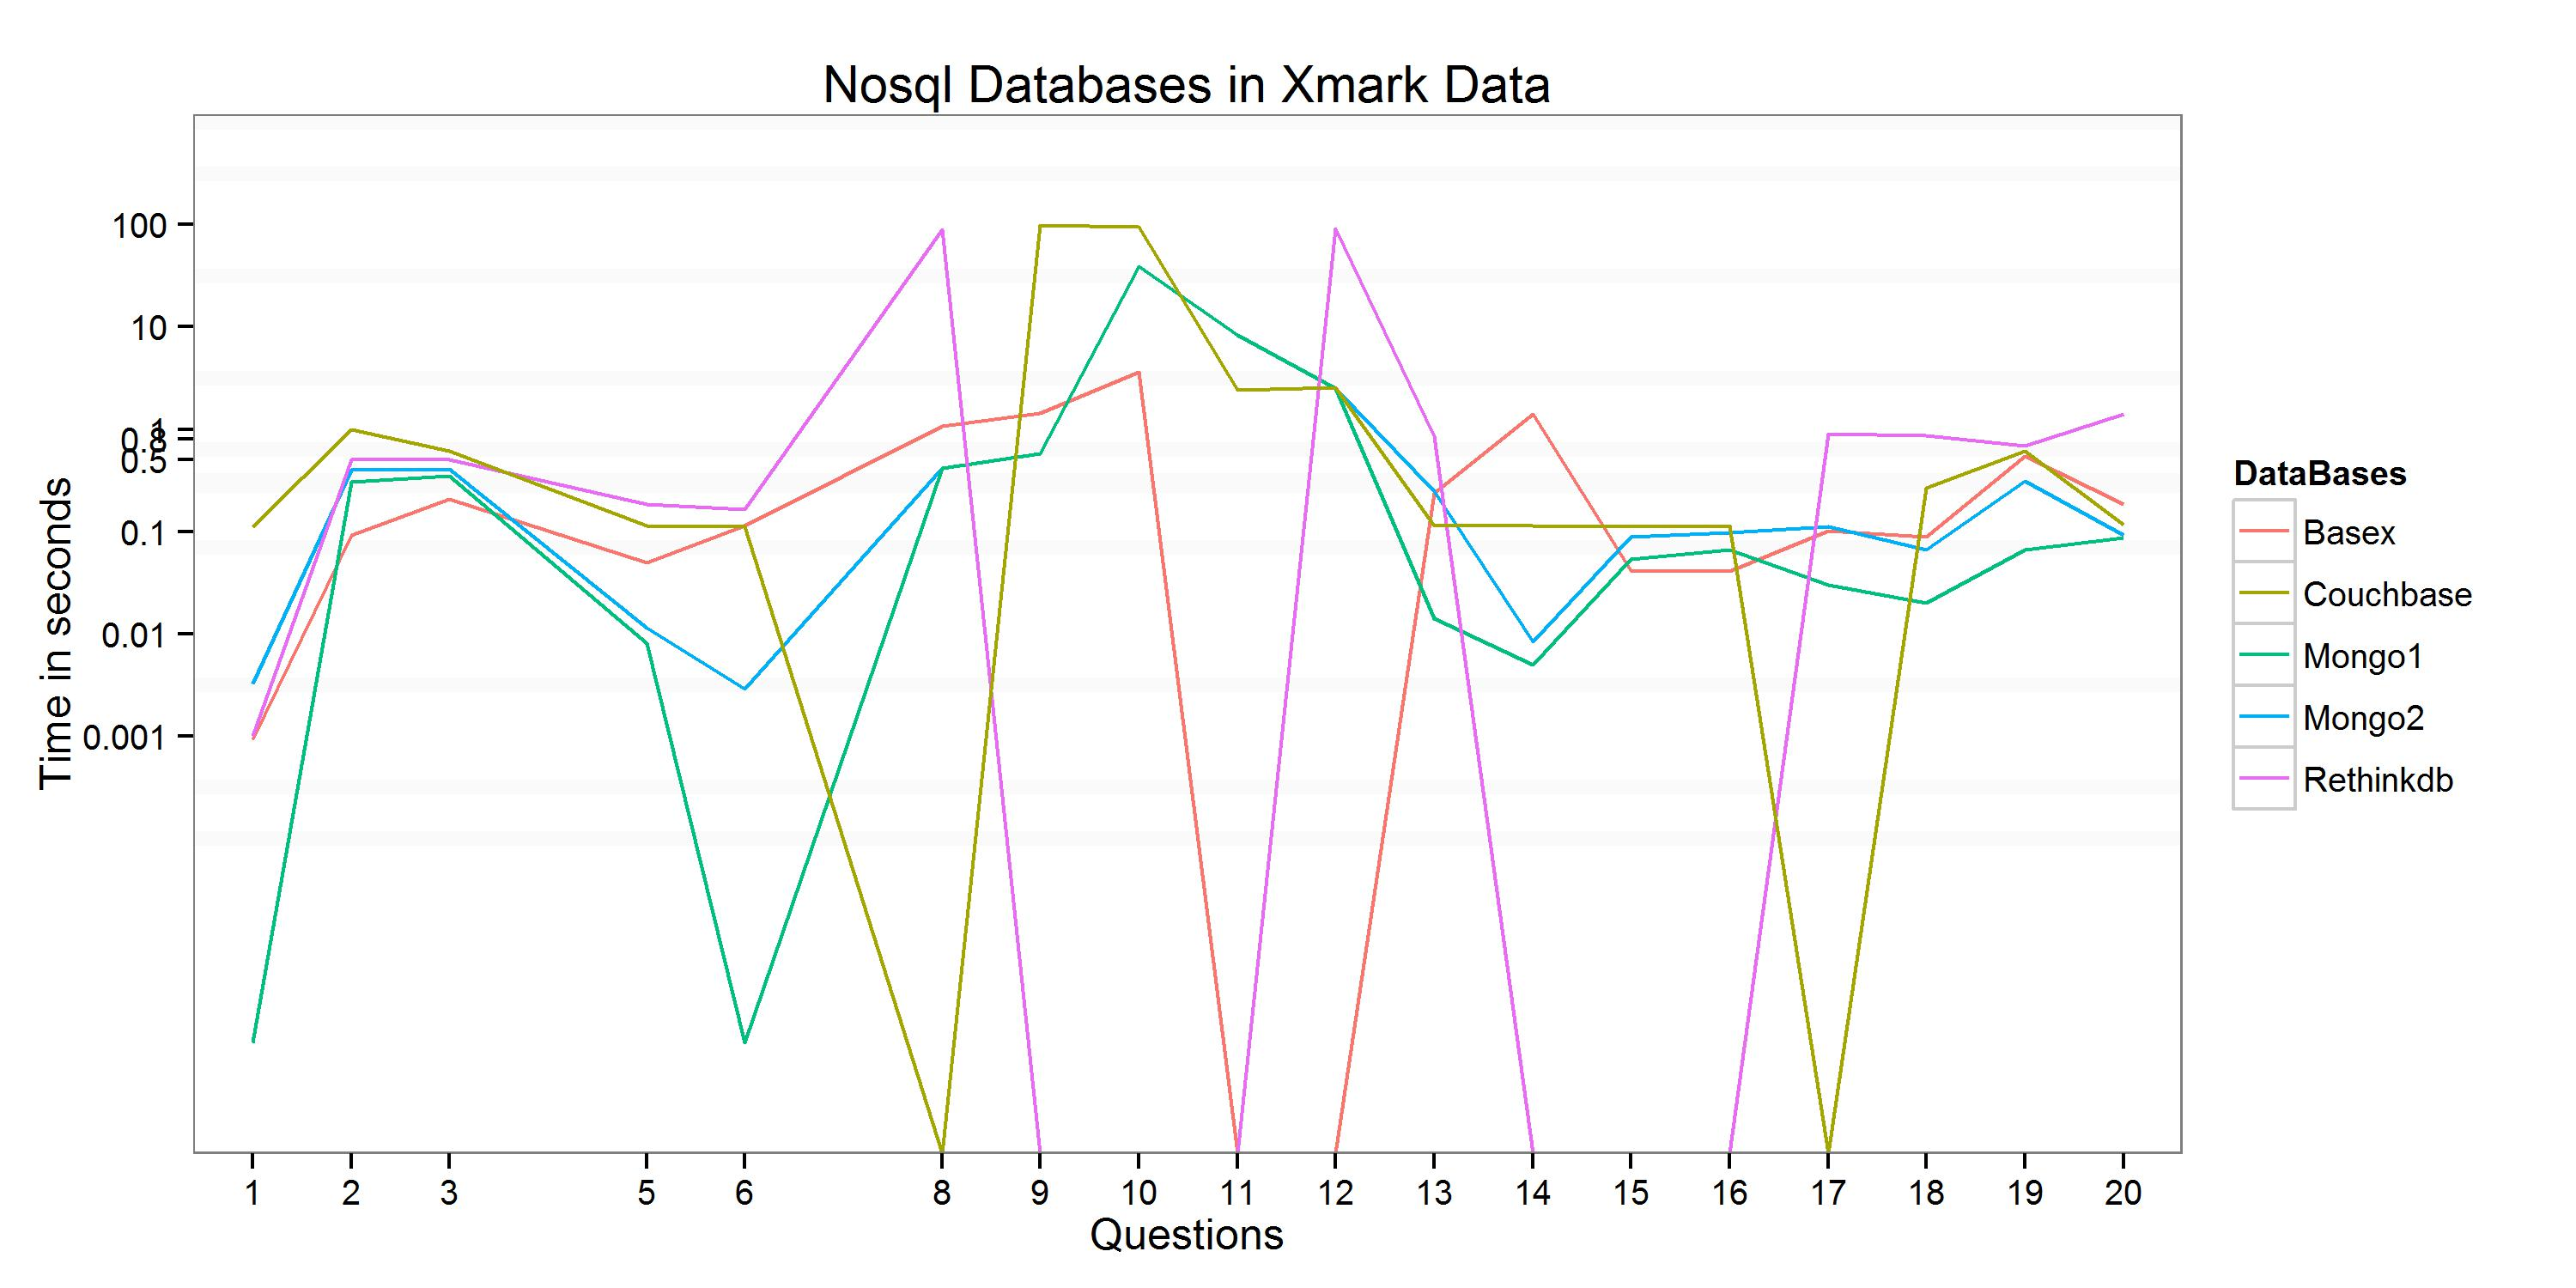
\includegraphics[width=0.9\textwidth]{img/Plot7}
	\caption{An overview of some important indexing structures developed over years}
	\label{trees}
\end{figure}

